I am working full-time at T-Mobile as a Cybersecurity Engineer and admitted in Ph.D. in Security program at UCCS. 
My research interest is in systems and software security area. 
I have done my undergrad from India in Computer Engineering and completed my Master’s in Cybersecurity \& Leadership from the University of Washington-Tacoma. 
\begin{figure}[h!]
\centering
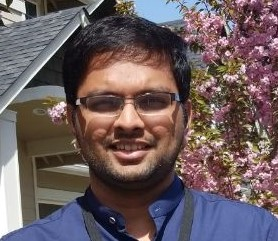
\includegraphics[scale=0.5]{parth_shah.jpg}
\caption{Photo of Parth}
\label{fig:profile}
\end{figure}
I have accumulated around 8 years of corporate experience in application/systems security working on various areas of secure software development lifecycle (SSDLC). 
I have also acquired some certifications along way such as CISSP, CCSK and CEH.  


My primary objective to pursue PhD is to become subject matter expert in systems and software security area. 
After the program, I would like to take up strategic technical leadership position with a better understanding and approach to the complex problems. 
I would also like to play a role in the betterment of academic-corporate partnership in future research areas.

Questions for Parth:\\
\textit{Question 1: }Prajjwal here, hi. Can you share one way in which academic-corporate partnerships can be made better given both have unique advantages when it comes to research?
